% !TEX root = ../thesis-sample.tex

\chapter{Multi-Vehicle Autonomous Exploration and Patrol} \label{chap:multivehicle}

This chapter covers a bidding-based formulation for multiple vehicles cooperating together in the context of autonomous exploration and patrol. We focus on a series of auctions to assign tasks, and consider dynamic obstacles, such as people, in large office-like environments using a receding-horizon framework.

\section{Bidding-Based Autonomous Exploration}

When exploring uncertain environments, robots can generate large maps much faster if they coordinate their efforts. However, the problem of determining a multi-vehicle exploration strategy is complicated and computationally expensive, but must be performed in real-time.

In this section, we formulate a cooperative and autonomous exploration scheme based on sequential auctions for maximizing map information gain. The first auction is based on the expected information gain presented in the prior section, scaled by travel distance. Once the winner of the first auction is determined, the map for bidding is updated based on the expected measurements of the first robot. The second auction for the remaining robots is determined by the information gain from the revised map that is further scaled by the travel distance and a penalty for collision-avoidance. This process is repeated until all robots are assigned tasks. 

\subsection{Objective Function for the First Auction}


Here, we describe how robots participate in the first auction for maximizing map information gain while accounting for travel time. The information gain \refeqn{ObjFunApproxCompleteCartesian} is computed for each candidate pose. Expected information gains may vary among the robots only if they have different sensor configurations. All expected information gains must be computed prior to the first auction.

Next, we describe how travel time is integrated into exploration. Considering that distances from current robot poses to candidate poses may differ greatly, accounting for these varying travel times properly is essential for exploration time efficiency. Travel distances are computed using Dijkstra's search to provide collision-free waypoints for each robot. There are two steps: first, generate a cost map from the robot location to each location on the 2D projected map. This provides the collision-free distances to all reachable locations on the map. Second, the waypoints from a candidate pose to the current robot pose are easily obtained along the cost map using steepest descent. 

Here, we define a bump function to account for varying travel distances from Dijkstra's search. Let the distance along the collision-free path from the $k$-th robot pose, namely $X_k$, to the $c$-th candidate pose, namely $X_c$, be denoted $d(X_k,X_c,m_\text{2D})\geq0$, which is taken from the cost map belonging to $X_k$. A continuous bump function is defined to account for traveling costs, and is composed of two parts.  

The first part of the bump function corresponds to short trajectories. Consider $d_\text{opt}$, the time-optimal distance that a robot may travel at full speed during the time between exploration updates. Here, we consider the case when $d(X_k,X_c,m_\text{2D})\leq d_\text{opt}$, i.e., the robot can completely traverse this distance during the allotted travel time. If $d(X_k,X_c,m_\text{2D})\ll d_\text{opt}$, then the robot is not moving at its full potential. This can be wasteful, because the robot tends to capture larger regions while moving. Therefore, it is desirable for $d(X_k,X_c,m_\text{2D})\rightarrow d_\text{opt}$, which corresponds to maximizing map coverage without time cost. The first part of the bump function is sinusoidal and is optimized at $d_\text{opt}$ to maximize robotic movement as
\begin{align}
\label{eqn:BumpFunIncreasing}
\mathcal B_1(d)=\frac12 f_\text{max}\left(1-\cos{\frac{d\pi}{d_\text{opt}}}\right),
\end{align}
where $f_\text{max}>0$ is the maximum value when $d(X_k,X_c,m_\text{2D})=d_\text{opt}$.

The second part of the bump function is defined over the domain where \\$d(X_k,X_c,m_\text{2D})>d_\text{opt}$ to minimize time required for $X_k$ to arrive at $X_c$, putting a penalty on traversing across the environment. This choice is beneficial to generating accurate local maps before exploring new regions. The second half is defined to be nonzero everywhere and is strictly decreasing as 
\begin{align}
\label{eqn:BumpFunDecreasing}
\mathcal B_2(d)=(f_\text{max}-f_\text{far})\exp\braces{-\beta(d_\text{opt}-d)^2}+f_\text{far},
\end{align}
where $f_\text{max}>f_\text{far}>0$ guarantees $\mathcal B_2>0$ such that $\mathcal B_2\rightarrow f_\text{far}$ as $d(X_k,X_c,m_\text{2D})\rightarrow\infty$ and $\beta>0$ assigns the rate of functional decrease relative to $f_\text{max}$ and $f_\text{far}$. Then, the complete bump function is defined as
\begin{align}
\label{eqn:BumpFun}
\mathcal B(d)=
\begin{cases}
    \mathcal B_1(d),		& \text{if }d\leq d_\text{opt},\\
    \mathcal B_2(d),         & \text{otherwise},
\end{cases}
\end{align}
which is illustrated in Fig. \ref{fig:nonzeroBumpFun}. % In short, the bump function prioritizes short movements to capture the local environment over long traversals for exploration time efficiency.

	\begin{figure}
		\centerline{
			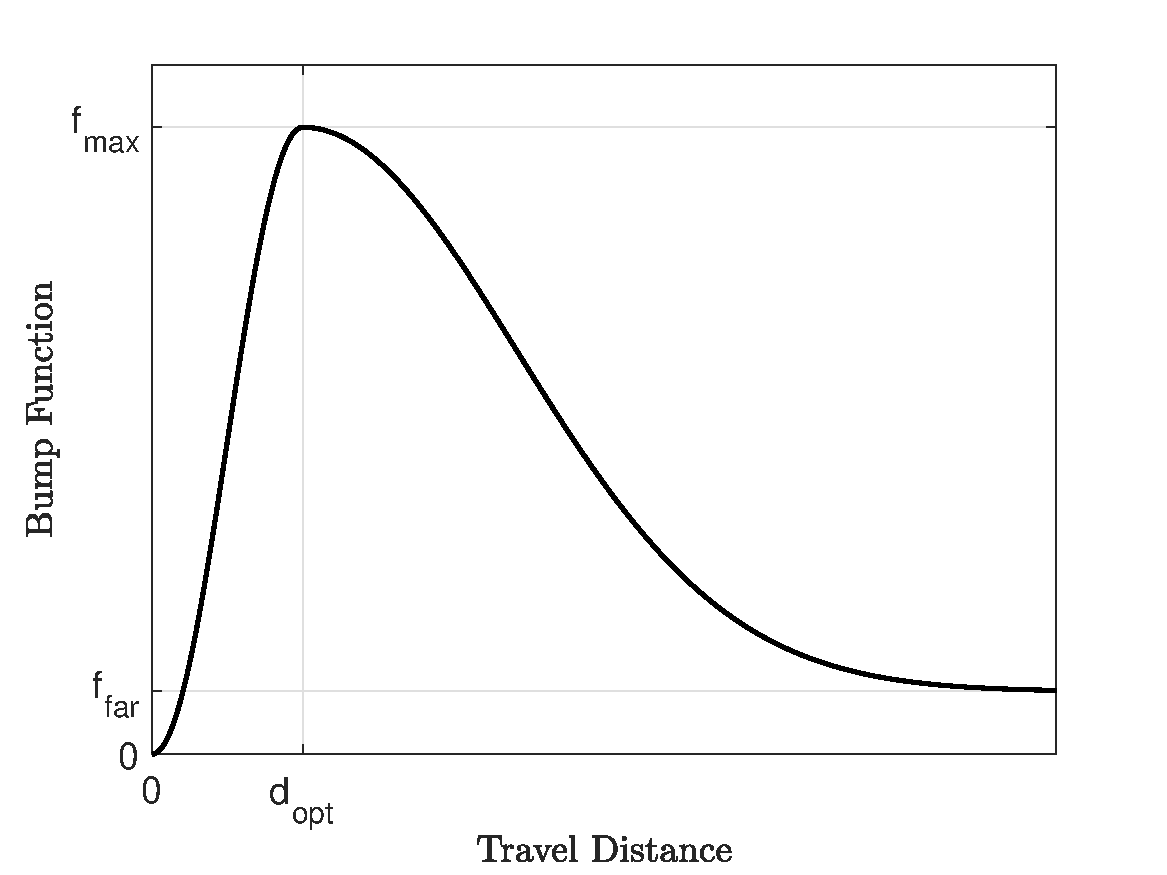
\includegraphics[width=0.9\columnwidth]{NonZeroBump.pdf}
		}
		\caption{The bump function is designed to promote travel distances close to $d_\text{opt}$ by multiplying this function by the expected information gain objective. Travel distances less than $d_\text{opt}$ are below the robot capabilities. Travel distances beyond $d_\text{opt}$ are beyond what the robot can reach within the minimum exploration computation time.}
		\label{fig:nonzeroBumpFun}
	\end{figure}
	
Then, using the information gain from \refeqn{expectedInfoGainRay} and considering the impact from travel distance from \refeqn{BumpFun}, the objective function for a single agent with respect to $X_{c}$ is
\begin{align}
\label{eqn:CandidateBidSingle}
\text{Obj}_\text{single}(X_k,X_c,m_\text{2D})&=\mathcal B(d(X_k,X_c,m_\text{2D}))\mathcal I(X_{c},m_\text{2D}).
%X_{k,c}^*&=\argmax_{X_c}{\ \mathcal B_{k,c}\mathcal I(X_c)},
\end{align}
Then, the optimal pose selection for the $k$-th agent is
\begin{align}
\label{eqn:OptPoseSingle}
X^*_{k}=\argmax_{X_c}\text{Obj}_\text{single}(X_k,X_c,m_\text{2D}).
\end{align}
Therefore, the bump function from \refeqn{BumpFun} prioritizes robotic movement within the local surrounding space before the robot moves across the map to distant regions, while still considering faraway pose candidates.

The first auction includes bids from all robots, and proceeds as follows. Let the set of all $n_R$ robots be denoted $\mathcal R=\braces{R_1,R_2,\dots,R_{n_R}}$ such that the $k$-th robot, namely $R_k$, bids $\text{Obj}_\text{single}(X^*_k,X_c,m_\text{2D})$ from \refeqn{CandidateBidSingle} and \refeqn{OptPoseSingle}. This is repeated for all $k$ such that $R_k\in\mathcal R$. The robot with the largest bid wins the first auction at index $k^*$, and is assigned to travel to $X^*_{k^*}$. Then, the remaining robots must account for the planned trajectory of the robot that won the first auction in subsequent auctions, described next.



\subsection{Objective Function for Subsequent Auctions}

\subsection{Receding Horizon Framework}

\subsection{Multi-Vehicle Exploration Numerical Simulation}
% Multi-vehicle ICRA figs 3-6 (remake fig. 5 with larger contrast)

\section{Multi-Vehicle Cooperative Patrol}

\subsection{Continuous-Time Markov Process for Cell Degradation}
% JINT18 fig. 3

\subsection{Multi-Vehicle Patrol Numerical Simulation}
% JINT18 fig. 10-13 (ref. ICRA fig 3 from above in this chapter)

\section{Conclusions}





